% !TEX TS-program = pdflatexmk
% !TEX root = EUDAQUserManual.tex
\documentclass[12pt, oneside, notitlepage, a4paper]{scrartcl}
\usepackage{epsfig, scrlayer-scrpage, graphicx, listings, microtype, setspace, upquote}
\usepackage[british]{babel}
\usepackage{hyperref} % must be the last package (apart from glossaries)
\usepackage[toc, nonumberlist]{glossaries} % must go after hyperref, so entries are clickable

\setcounter{secnumdepth}{3}
\setcounter{tocdepth}{2}

\setlength{\parindent}{0em}
\setlength{\parskip}{0ex plus0.5ex minus0ex}
\pagestyle{scrheadings}

\def\subsectionautorefname{section}
\def\subsubsectionautorefname{section}
%\let\stdsection\section
%\renewcommand\section{\newpage\stdsection}

% Some useful commands
\newcommand*\micron{\ensuremath{\mu\mathrm{m}}}
\newcommand*\micro{\ensuremath{\mu}}
\newcommand*\square{\ensuremath{^2}}
\newcommand*\degree{\ensuremath{^\circ}}
\newcommand*\lt{\ensuremath{<}}
\newcommand*\gt{\ensuremath{>}}
\newcommand*\x{\ensuremath{\times}}
\newcommand*\param[1]{\ensuremath{\langle}#1\ensuremath{\rangle}}

\newcommand*\ttitem[1]{\item[\texttt{#1}\,:]}
\newcommand*\ccitem[1]{\item[]\lstinline[style=shaded,language=C++]{#1}}
%\lstMakeShortInline[style=plain,language=C++]@
\newcommand*\inline[2][C++]{\lstinline[style=plain,language=#1]{#2}}

\newcommand*\myinputlisting[3][C++]{
  %% Latest version available at:\\
  %% \textls[#2]{\url{https://github.com/eudaq/eudaq/blob/master/#3}}

\lstinputlisting[style=full, language=#1]{../../#3}
%% \rule[\baselineskip]{\textwidth}{1pt}
}

\lstnewenvironment{listing}[1][C++]{\lstset{style=shaded,language=#1}}{}

\newenvironment{myitemize}
{\begin{itemize}%
  \setlength{\itemsep}{0.1\baselineskip}%
  \setlength{\parskip}{0pt}%
  \setlength{\parsep}{0pt}}
{\end{itemize}}
\newenvironment{mydescription}
{\begin{description}%
  \setlength{\itemsep}{0.1\baselineskip}%
  \setlength{\parskip}{0pt}%
  \setlength{\parsep}{0pt}}
{\end{description}}

\renewcommand*\headfont{\normalfont}

\renewcommand*\glsgroupskip{}
\renewcommand*{\glspostdescription}{.\vspace{-0.5\baselineskip}}
\makeglossaries

%\glsdisablehyper
%\defglsdisplay{\cooltooltip[1,1,0.9][1,1,1]{Glossary}{a #2}{}{b #2}{#1}}
%\renewcommand{\glsdisplay}[4]{%
%   \cooltooltip[1,1,1][1,1,0.9]{Definition}{#2}{}{#2}{#1#4}%
%} 

\lstset{
    %basicstyle=\ttfamily
    keywordstyle=\color[rgb]{0,0,0.8},
    %identifierstyle=\color[rgb]{0,0,0},
    commentstyle=\color[rgb]{0,0.4,0},
    stringstyle=\color[rgb]{0.4,0,0.8},
    showstringspaces=false,
    basewidth=1.2ex,
    numberstyle=\footnotesize\color[rgb]{0.6,0.6,0.6},
    stepnumber=1,
    numbersep=10pt,
    tabsize=2,
    breaklines=true,
    prebreak = \raisebox{0ex}[0ex][0ex]{\color[rgb]{0.6,0.6,0.6}\ensuremath{\hookleftarrow}},
    breakatwhitespace=true,
    %aboveskip={1.5\baselineskip},
    columns=fixed,
    upquote=true,
    extendedchars=false,
    framerule=0pt,
    belowskip={0.5\baselineskip},
}
\lstdefinestyle{plain}{
    basicstyle=\normalsize\ttfamily,
    numbers=none,
    frame=none,
    %belowskip={0.5\baselineskip},
    backgroundcolor={},
}
\lstdefinestyle{shaded}{
    basicstyle=\small\ttfamily,
    numbers=none,
    frame=single,
    backgroundcolor=\color[rgb]{1,0.98,0.95},
}
\lstdefinestyle{full}{
    basicstyle=\small\ttfamily,
    numbers=left,
    frame=single,
    %belowskip={\baselineskip},
    backgroundcolor=\color[rgb]{1,1,0.95},
}

\lstdefinestyle{cpp}{
    language=C++, 
    morekeywords={override, final},
    basicstyle=\small\ttfamily,
    numbers=left,
    frame=single,
    %belowskip={\baselineskip},
    backgroundcolor=\color[rgb]{1,1,0.95},
    %% texcl=true,
    rangeprefix=//----------DOC-MARK-----,
    rangesuffix=-----DOC-MARK----------,
    includerangemarker=false,
    columns=flexible,
    %% escapeinside={//TODO}{.},
}


\lstdefinelanguage{conf}{
    otherkeywords={=},
    alsoletter={[},
    alsoletter={]},
    moredelim=[s][keywordstyle]{[}{]},
    comment=[l]{\#},
    %morecomment=[l]{\;},
    %string=[s]',
    %morestring=[s]",
}
\lstdefinelanguage{mybash}[]{bash}{
    deletekeywords={test,read},
    morekeywords={svn,make,chown,chmod},
    %keywordsprefix={./},
    moredelim=[is][keywordstyle]{$[}{]$},
}


% Insert EUDET document number here:
\newcommand*\EUDETnum{EUDAQ User Manual}

% PDF info and link colours
\hypersetup{
  pdftitle={EUDAQ User Manual},
  pdfauthor={EUDAQ Development Team},
  pdfsubject={EUDAQ},
  pdfkeywords={EUDET, EUDAQ, Software, User Manual},
  colorlinks=true,
  linkcolor=black, % \ref \autoref \pageref
  citecolor=blue, % \cite
  urlcolor=blue, % \url \href (external)
  filecolor=blue, % \href (local file)
}

% Load glossary
\loadglsentries{src/glossary.tex}

% Headers and Footers
\titlehead{\EUDETnum}
\lehead{\EUDETnum}
\lohead{\EUDETnum}
\automark{section}
\rehead{\headmark}
\rohead{\headmark}
\chead{}
\cfoot{\pagemark}

% Title info
\subject{
\begin{center}
\includegraphics[width=0.1\textwidth]{src/images/logo_eudet} \includegraphics[width=0.3\textwidth]{src/images/AIDA_logo_medium} 
%
\includegraphics[width=0.3\textwidth]{src/images/logo_aida2020}
\vspace{.5cm}\\
\includegraphics[width=0.6\textwidth]{src/images/eudaq_logo}
\end{center}
}
\title{\Large EUDAQ User Manual} 
\author{\normalsize EUDAQ Development Team}
\input{src/version.tex} % defines the \CMakeLibVersion command which is
                    % set by CMake to the current EUDAQ version number
                    % (with git hash tag)
\date{\normalsize Last update on October 2016 \\  %\today
for EUDAQ version v1.7} %\CMakeLibVersion}

\begin{document}

% Title page
\maketitle
\begin{abstract}
\noindent
This document provides an overview of the EUDAQ software,
the data acquisition framework used by the EUDET JRA1 beam telescope.
It describes how to install and run the DAQ system and use many of the included utility programs,
and how users may integrate their systems into the EUDAQ framework
by writing their own Producer and DataConverterPlugin,
thus allowing them to take advantage of the EUTelescope analysis framework.
\end{abstract}
\newpage

% Contents
% Condense slightly to fit on one page
\begin{spacing}{0.92}
\tableofcontents
\end{spacing}

% Main sections
\include{src/License}
% !TEX root = EUDAQUserManual.tex
\section{Introduction}
The EUDAQ software is a data acquisition framework, written in C++,
and designed to be modular and portable, running on Linux, Mac OS X, and Windows.
It was written primarily to run the EUDET-type beam telescope~\cite{Roloff:2009zza,Jansen:2016},
but is designed to be generally useful for other systems.

The hardware-specific parts are kept separate from the core,
so that the core library can still be used independently.
For example, hardware-specific parts are two components for the EUDET-type beam telescope: \gls{TLU} and \gls{NI} for Mimosa 26 sensor read out.

The raw data files generated by the DAQ can be converted to the \gls{LCIO} format,
allowing for analysing the data using the EUTelescope package \cite{eutel2008}.

\subsection{Architecture}
It is split into a number of different processes,
each communicating using TCP/IP sockets (compare \autoref{fig:DAQ}).
A central Run Control provides an interface for controlling the whole DAQ system;
other processes connect to the Run Control to receive commands and to report their status.

\begin{figure}[htb]
  \begin{center}
    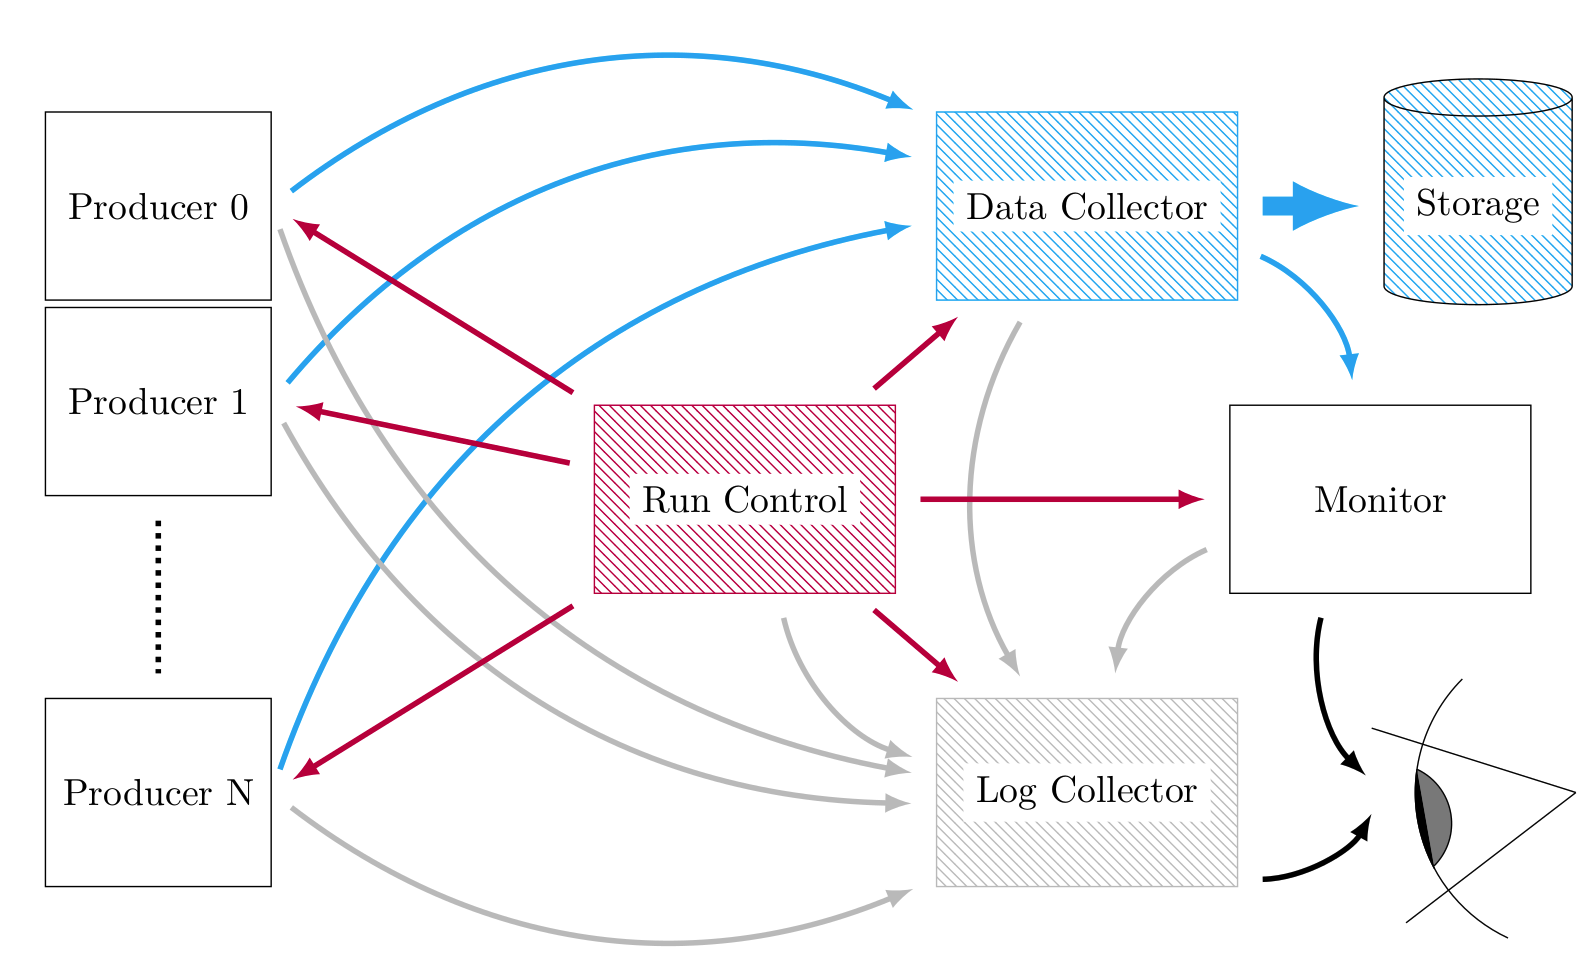
\includegraphics[width=0.9\textwidth]{src/images/eudaq_working_principle}
    \caption{Schematic of the EUDAQ architecture \cite{Spannagel:2016}.}
    \label{fig:DAQ}
  \end{center}
\end{figure}

Each hardware that produces data (e.g. the \gls{TLU}, the \gls{NI}, or a \gls{DUT}) will have a Producer process (on the left in \autoref{fig:DAQ}).
This will initialize, configure, stop and start the hardware by receiving the commands from the Run Control (red arrows), read out the data and send it to the Data Collector (blue arrows).

The Data Collector receives all the data streams from all the Producers,
and combines them into a single stream that is written to disk (Storage).
It writes the data in a native raw binary format,
but it can be configured to write in other formats, such as \gls{LCIO}.

The Log Collector receives log messages from all other processes (grey arrows),
and displays them to the user, as well as writing them all to file.
This allows for easier debugging, since all log messages are stored together in a central location.

The Monitor reads the data file and generates online-monitoring plots for display.
In the schematic it is shown to communicate with the Data Collector via a socket,
but it actually just reads the data file from disk.

\subsection{Directory and File Structure}
The EUDAQ software is split into several parts that can each be compiled independently,
and are kept in separate subdirectories.
The general structure is outlined below:

\begin{myitemize}
\item \texttt{main}
  contains the core EUDAQ library with the parts that are common to most of the software,
  and several command-line programs that depend only on this library.
  All definitions in the library should be inside the \texttt{eudaq} namespace.
  It is organised into the following subdirectories:
  \begin{myitemize}
  \item \texttt{lib/src}
    contains the library source code,
  \item \texttt{exe/src}
    contains the (command line) executables source code,
  \item \texttt{include}
    contains the header files inside the \texttt{eudaq} subdirectory (to match the namespace),
  \end{myitemize}
\item \texttt{gui}
  contains the graphical programs that are built with Qt, such as the RunControl and LogCollector.
\item \texttt{producers}
  contains all (user-provided) producers shipped with the EUDAQ
  distribution, for example:
  \begin{myitemize}
\item \texttt{tlu}
  contain the parts that depend on the \gls{TLU}.
\item \texttt{ni}
  contain the parts that depend on the \gls{NI} system for Mimosa 26 read out.
\item e.g. \texttt{depfet}, \texttt{fortis}, \texttt{taki}\ldots{}
  contain the code for third-party producers that have been used with
  EUDET-type beam telescopes.
  \end{myitemize}
\item \texttt{extern}
  stores external software that is not part of EUDAQ itself, but that is needed by EUDAQ in some cases,
  such as the \texttt{ZestSC1} driver and the \texttt{tlufirmware} for the \gls{TLU}.
% and the Tsi148 VME driver.
\item \texttt{bin} and \texttt{lib}
  contain the compiled binaries (executables and libraries) generated from the other directories.
\item \texttt{conf}
  contains configuration files for running the beam telescope.
\item \texttt{data} and \texttt{logs}
  are directories for storing the data and log files generated while running the DAQ.
\item \texttt{doc}
  contains documentation, such as this manual.
\end{myitemize}

Each directory containing code has its own \texttt{src} and \texttt{include} subdirectories,
as well as a local \texttt{CMakeLists.txt} file containing the rules
for building that directory using \texttt{CMake}.
Header files usually have a \texttt{.hh} extension so that they can be automatically recognised as C++
(as opposed to C), and source files have either \texttt{.cc} for parts of a library or \texttt{.cxx} for executables.

Each directory can contain a \texttt{README.md} file for brief documentation for this specific part, e.g.  
as installation advice. 
Using the \texttt{*.md} file ending allows for applying the Markdown language \cite{markdownWWW}. 
Accordingly, content will be formatted on the the GitHub platform, where the code is hosted online.

% !TEX root = EUDAQUserManual.tex
\section{Installing EUDAQ}

The installation is described in four steps:%
\footnote{A quick installation manual is also described in the \texttt{README.md}, e.g. \url{https://github.com/eudaq/eudaq/blob/v1.6-dev/README.md}.}
\begin{enumerate}
\item Installation of (required) prerequisites
\item Downloading the source code (GitHub)
\item Configuration of the code (CMake)
\item Compilation of the code
\end{enumerate}

If you occur problems during the installation process, please have a look into the issue tracker on GitHub.%
\footnote{Go to \url{https://github.com/eudaq/eudaq/issues}} 
Here you can search, if your problem had already been experienced by someone else, or you can open a new issue (see \autoref{sec:reporting}).

\subsection{Installation of prerequisites}

EUDAQ has few dependencies on other software, but some features do rely on other packages:
\begin{itemize}
\item To get the code and stay updated with the central repository on GitHub git is used.
\item To configure the EUDAQ build process, the CMake cross-platform, open-source build system is used.
\item To compile EUDAQ from source code requires a compiler that implements the C++11 standard.
\item The libusb library is needed to communicate over USB with a \gls{TLU} \cite{Cussans2009}.
\item Qt is required to build GUIs of the e.g. Run Control Log Collector. 
\item ROOT is required for the Online Monitor.
\end{itemize}

\subsubsection{Git}
Git is a free and open source distributed version control and is available for all of the usual platforms \cite{gitWWW}. 
It allows for local version control and repositories, but also communicating with central online repositories like GitHub.
   
In order to get the EUDAQ code and stay updated with the central repository on GitHub git is used (see \autoref{sec:downloadingEUDAQ}).
But also for developing the EUDAQ code having different versions (tags) or branches (development repositories), git is used (see \autoref{sec:contributing}).


\subsubsection{CMake (required)}
In order to automatically generate configuration files for the build process of EUDAQ both compiler and platform independent, the CMake build system is used.

CMake is available for all major operating systems from \url{http://www.cmake.org/cmake/resources/software.html}. On most Linux distributions, it can usually be installed via the built-in package manager (aptitude/apt-get/yum etc.) and on OSX using packages provided by e.g. the MacPorts or Fink projects.

\subsubsection{C++11 compliant compiler (required)}
The compilation of the EUDAQ source code requires a C++11 complianti compiler and has been tested with GCC (at least version 4.8), Clang (at least version 3.1), and MSVC (Visual Studio 2012 and later) on Linux, OS X and Windows.

If you are using Scientific Linux, please install the \emph{Developer Toolset} available e.g. from \url{http://linux.web.cern.ch/linux/devtoolset/} to get access to a GCC version which fully implements C++11, e.g. on SL6 do
\begin{listing}[mybash]
scl use devtoolset-1.1 bash
\end{listing}
and cmake and install in this bash.

\subsubsection{libusb (for the EUDET TLU)}
In order to communicate over USB with a \gls{TLU}, the libusb library is needed.
Therefore, if you want to compile the \texttt{tlu} subdirectory, you should make sure that libusb is properly installed.

On Mac OS X, this can be installed using Fink or MacPorts.
If using MacPorts you may also need to install the \texttt{libusb-compat} package.

On Linux it may already be installed,
otherwise you should use the built-in package manager to install it.
Make sure to get the development version, which may be named \texttt{libusb-devel} instead of simply \texttt{libusb}, e.g. on Ubuntu: 
\begin{listing}[mybash]
sudo apt-get install libusb-dev 
\end{listing}

On Windows, libusb is only needed if compiling with cygwin,
in which case you should use the cygwin installer to install libusb.
Otherwise libusb is not needed, as the included ZestSC1 libraries should work as they are.

\subsubsection{ZestSC1 drivers and TLU firmware files (for the EUDET TLU)}
Additonally to the libusb library, the EUDET \gls{TLU} producer requires the
ZestSC1 driver package and the FPGA firmware bitfiles. 
These are available to download via AFS from DESY. 
If AFS is accessible on the machine when CMake is run, the necessary files will be installed
automatically.
Otherwise, manually copy full folder with sub-directories from
\begin{itemize}
\item \texttt{/afs/desy.de/group/telescopes/tlu/ZestSC1} and
\item \texttt{/afs/desy.de/group/telescopes/tlu/tlufirmware}
\end{itemize}
into the \texttt{extern} subfolder in your EUDAQ source directory.


\subsubsection{Qt (for GUIs)}
The graphical interface of EUDAQ uses the Qt graphical framework.
In order to compile the \texttt{gui} subdirectory, you must therefore have Qt installed.
It is available in most Linux distributions as the package \texttt{qt4-devel} or  \texttt{qt5-devel}
but make sure the version is at least 4.4, since there are a few issues with earlier versions.

If the included version is too old, or on other platforms,
it can be downloaded from \url{http://qt.nokia.com/downloads}.
Select the LGPL (free) version, then choose the complete development environment
(it may also work with just the framework, but this is untested).
Make sure the \texttt{QTDIR} environment variable is set to the Qt installation directory,
and the \texttt{\$QTDIR/bin} directory is in your path.

If you are using OSX, the easiest way to install Qt is using the
packages provided by the MacPorts project (\url{http://www.macports.org/}).

\subsubsection{ROOT (for Monitor)}
\label{sec:Root}
The Online Monitor, as well as a few command-line utilities (contained in the \texttt{root} subdirectory), use the ROOT package for histogramming.
It can be downloaded from \url{http://root.cern.ch} or installed via
your favorite package manager.

Make sure ROOt's \texttt{bin} subdirectory is in your path, so that the \texttt{root-config} utility can be run.
This can be done by sourcing the \texttt{thisroot.sh} (or \texttt{thisroot.ch} for csh-like shells)
script in the \texttt{bin} directory of the ROOT installation:
\begin{listing}[mybash]
source /path-to/root/bin/thisroot.sh
\end{listing}

\subsubsection{LCIO / EUTelescope (for converting/analysis)}
\label{sec:LCIO-EUTel}
To enable the writing of \gls{LCIO} files, or the conversion of native files to \gls{LCIO} format,
EUDAQ must be linked against the \gls{LCIO} and EUTelescope libraries.
Detailed instructions on how to install both using the
\texttt{ilcinstall} scripts can be found at \url{http://eutelescope.web.cern.ch/content/installation}.

The \texttt{EUTELESCOPE} and \texttt{LCIO} environment variables should be set to the
installation directories of EUTelescope and LCIO respectively.
This can be done by sourcing the \texttt{build\_env.sh} script as follows:
\begin{listing}[mybash]
source /path-to/Eutelescope/build_env.sh
\end{listing}

%%%%%%%%%%%%%%%%%%%%%%%%%%%%%%%%%%%%%%%%%%%%%%%%%%%%%%%%%%%
\subsection{Download the source code from GitHub}
\label{sec:downloadingEUDAQ}

The EUDAQ source code is hosted on GitHub \cite{githubEUDAQ}. 
Here, we describe how to get the code and install a stable version release. 
In order to get information about the work flow of developing the EUDAQ code, please find the relevant information in see \autoref{sec:contributing}.

\subsubsection{Downloading the code (clone)}
We recommend to obtain the software by using git,
since this will allow you to easily update to newer versions.
The source code can be downloaded with the following command:
\begin{listing}[mybash]
git clone https://github.com/eudaq/eudaq.git eudaq
\end{listing}
This will create the directory \texttt{eudaq}, and download the latest
version into it. 

\textit{Note:} Alternatively and without version control, you can also download a zip/tar.gz file of EUDAQ releases (tags) from \url{https://github.com/eudaq/eudaq/releases}. 
By downloading the code, you can skip the next two subsections. 

\subsubsection{Changing to a release version (checkout)}
After cloning the code from GitHub, your local EUDAQ version is on the master branch (check with \texttt{git status}).  
For using EUDAQ without development or for production environments (e.g. at test beams), we strongly recommend to use the latest release version. 
Use 
\begin{listing}[mybash]
git tag 
\end{listing}
in the repository to find the newest stable version as the last entry.
In order to change to this version in your local repository, execute e.g. 
\begin{listing}[mybash]
git checkout v1.6.0
\end{listing}
to change to version v1.6.0.

\subsubsection{Updating the code (fetch)}
If you want to update your local code, e.g to get the newest release versions, execute in the \texttt{eudaq} directory: 
\begin{listing}[mybash]
git fetch
\end{listing}
and check for new versions with \texttt{git tag}. 


\subsection{Configuration via CMake}
CMake supports out-of-source configurations and builds -- just enter
the './build' directory and run CMake, i.e.
\begin{listing}[mybash]
cd build
cmake ..
\end{listing}

CMake automatically searches for all required packages and verifies
that all dependencies are met using the \texttt{CMakeLists.txt} script in the
main folder. By default, only the central shared library, the main
executables and (if Qt4 or Qt5 have been found) the graphical user
interface (GUI) are configured for compilation. You can modify this
default behavior by passing the \texttt{BUILD\_[name]} option to
CMake where \texttt{[name]} refers to an optional component, e.g.
\begin{listing}[mybash]
cmake -D BUILD_gui=OFF -D BUILD_tlu=ON ..
\end{listing}
to disable the GUI but enable additionally the TLU producer and
executables.

The corresponding settings are cached, so that they will be again used
next time CMake is run.

Some of the optional packages and producers include:
\begin{description}

\ttitem{main}
The common library, and some command-line programs that depend on only this library

\ttitem{tlu}
The \gls{TLU} library, and the command-line programs that depend on
it. Requires libusb, ZestSC1 drivers, and the TLU firmware files.

\ttitem{gui}
The graphical parts of the DAQ, such as the Run Control and Log
Collector. Require Qt to be installed.

\ttitem{onlinemon}
The Root Online Monitor. Requires Root to be installed.

\ttitem{nreader}
The native reader Marlin processor used for data conversion into LCIO
by EUTelescope. Requires LCIO and EUTelescope to be installed.

\texttt{manual}
This manual compiled from its \LaTeX sources. Requires a working
\LaTeX installation.

\end{description}

The producers are stored in the \texttt{./producer} subdirectory and
include: \texttt{altro}, \texttt{altroUSB}, \texttt{depfet},
\texttt{fortis}, \texttt{mimoroma}, \texttt{mvd},
\texttt{pixelmanproducer}, and \texttt{taki}. These are
user-contributed producers for specific detectors inside the EUDET
telescope.  They should not be compiled unless needed.

A short description of selected producers:
\begin{description}
\item{tlu}
\item{ni}
\end{description}



To install the binaries and the library outside the source tree, you
need to set the \texttt{INSTALL\_PREFIX} option, e.g.
\begin{listing}[mybash]
cmake -D INSTALL_PREFIX=/usr/local ..
\end{listing}
to install the executables into the \texttt{bin} and the library into \texttt{lib} subdirectories of \texttt{/usr/local}.

If you ever need to, you can safely remove all files from the build folder
as it only contains automatically generated files. Just run
\begin{listing}[mybash]
cd build
rm -rf *
\end{listing}
to start from scratch.


\subsection{Compilation}

\subsubsection{Compilation on Linux/OSX}
You should just have to run the command:
\begin{listing}[mybash]
make install
\end{listing}

from the top EUDAQ directory to compile the common library,
along with some command-line programs (the contents of the \texttt{./main/exe} subdirectory).
If other parts are needed, you can specify them as arguments to the
CMake command during the configuration step.

The executable binaries and the common shared library will be installed by default into the
\texttt{bin} and \texttt{lib} directories in the source tree,
respectively. If you would like to install into a different location,
please set the respective parameter during the CMake configuration.

\subsubsection{Setup and Compilation on Windows using Visual~Studio}

This section gives a short overview on the steps needed to compile the
project under Windows (tested under Windows 7, 32-bit). For a more
detailed introduction to the Windows build system and Visual~Studio
project files see the appendix~\ref{app:compileOnWindows} on
page~\pageref{app:compileOnWindows}.

\begin{itemize}
\item Prerequisites: 
\begin{itemize}
\item Download Qt4 or Qt5:
\item Download and install the pthreads library (pre-build binary from
  \url{ftp://sources.redhat.com/pub/pthreads-win32}) into either
  \texttt{c:\\pthreads-w32} or \texttt{./extern/pthreads-w32}
\item Download Visual Studio Express Desktop (e.g. 2013 Version):
  \url{http://www.microsoft.com/en-us/download/details.aspx?id=40787}
\end{itemize}

\item Start the Visual Studio \emph{Developer Command Prompt} from the
  Start~Menu entries for Visual~Studio (Tools subfolder) which opens a
  \texttt{cmd.exe} session with the necessary environment variables
  already set. If your Qt installation has not been added to the
  global \texttt{\%PATH\%} variable, you need to execute the \texttt{qtenv2.bat} batch file (or similar) in the Qt folder, e.g.
  
  \begin{listing}[mybash]
C:\Qt\Qt5.1.1\5.1.1\msvc2012\bin\qtenv2.bat
\end{listing}
Replace "5.1.1" with the version string of your Qt installation.

\item Now clone the EUDAQ repository (or download using GitHub) and enter the build directory on the prompt, e.g. by entering

  \begin{listing}[mybash]
cd c:\Users\[username]\Documents\GitHub\eudaq\build
\end{listing}

\item Configuration: Now enter

  \begin{listing}[mybash]
cmake ..
\end{listing}

to generate the VS project files.

\item Compile by calling
  \begin{listing}[mybash]
MSBUILD.exe EUDAQ.sln /p:Configuration=Release
\end{listing}
or install into \texttt{eudaq\\bin} by running
  \begin{listing}[mybash]
MSBUILD.exe INSTALL.vcxproj /p:Configuration=Release
\end{listing}
\item This will compile the main library and the GUI; for the remaining processors, please check the individual documentation.
\end{itemize}

Note on ``\emph{moc.exe - System Error: The program can't start
  because MSVCP110.dll is missing from your computer}'' errors: when using Visual~Express~2013 and \texttt{pthreads-w32} 2.9.1, you might require ``Visual C++ Redistributable for Visual Studio 2012'': download (either x86 or x64) from \url{http://www.microsoft.com/en-us/download/details.aspx?id=30679} and install.


% !TEX root = EUDAQUserManual.tex
\section{Running EUDAQ}
This section will describe running the DAQ system, mainly from the point of view of EUDET-type beam telescope \cite{telescopeWikiUserManual} operated together with \gls{DUT}s.
However, this description can be applied to DAQ system in general.

All executable programs from the different subdirectories are placed inside the \texttt{bin} subdirectory, and should be run from here. They should all accept a \texttt{-h} (or \texttt{--help}) command-line parameter, which will provide a summary of possible different command-line options.

\subsection{Preparation}
Some preparation is needed to make sure the environment is set up correctly and
the necessary TCP ports are not blocked before the DAQ can run properly.

\subsubsection{Directories}
EUDAQ expects two directories that will be used to store data files and log files.
These can be directories or symbolic links to other directories.

Firstly, inside the \texttt{eudaq} directory, there should be a directory (or a symbolic link) called \texttt{data}.
This will contain the data files written by the Data Collector, as well as a file containing the last run number,
so that it will continue incrementing even when the DAQ is restarted. 
Secondly, there should be a directory (or symbolic link) called \texttt{logs}.
This will be used by the Log Collector to store log files containing all the log messages received.

\subsubsection{Hostnames}
EUDAQ processes communicate between themselves using TCP/IP sockets.
When processes are started, they need to know where the Run Control runs.
There is no completely fool-proof way of determining this,
so processes look at the environment variable \texttt{\$HOSTNAME}.

Usually, this should be the DNS name of the machine it is running on, but in some cases it may not work correctly.
If this is the case, it may be necessary to set this variable manually, either to the real host name
or the machine's IP address. 
In the case, that all the processes will be running on the same computer, the host name can be set to \texttt{localhost} which correspons do the IP adress \texttt{127.0.0.1}.

Depending on the operating system and the command shell, you can set the host name by
\begin{itemize}
\item for bash-like shells: \inline[mybash]{export HOSTNAME=name}
\item for csh-like shells: \inline[csh]{setenv HOSTNAME name}
\item for Windows comman lines / scripts: \inline[mybash]{set HOSTNAME=name}
\end{itemize}
where \texttt{name} is the name or the IP adress.

Note: It is recommended to set the host name to the (local) IP adress. 
This method is approved and working at the EUDET-type telescopes at DESY and CERN.


\subsubsection{Ports and firewall}
The different processes communicate between themselves using TCP/IP sockets.
If a firewall is running, it may block these connections,
especially if the processes are running on different computers.
If all the processes will be run from the same computer,
then it is probably not necessary to do anything.
If a port is blocked, you will see an error message similar to the following
when attempting to start some programs:
\begin{listing}[]
Are you sure the server is running? - Error 61 connecting to localhost:44000: Connection refused
\end{listing}

The ports can be configured when calling the the processors on the command line (see below), but the default and usually free port numbers are:
\begin{description}

\ttitem{44000}
This is the port used to send commands from the Run Control.

\ttitem{44001}
This port is used to send data from the producers to the Data Collector.

\ttitem{44002}
This port is used to send log messages from all processes to the Log Collector.

\end{description}

If processes will be running on different computers,
then these ports should be opened up in the firewall.
The method for doing this depends on the Operating System used,
and is outside the scope of this manual.


\subsubsection{TLU permissions}\label{sec:TLUperm}
If you are not using a TLU conencted to a Linux OS, you may skip this part.

On many Linux distributions, the device node used to communicate over the USB bus is only
accessible by a user having root rights by default (\texttt{sudo ...}).
To set the correct permissions when a \gls{TLU} is
connected, you need to add a \texttt{udev} rule: as a root user, 
create the file \texttt{/etc/udev/rules.d/54-tlu.rules} and add
the following lines:
\begin{listing}
# for Debian
ACTION=="add", DRIVERS=="?*",  ATTR{idVendor}=="165d", ATTR{idProduct}=="0001",  MODE="0666"
\end{listing}
in case you are using a debian-based distribution such as Ubuntu.
\begin{listing}
# for Red Hat, e.g. SL5
SYSFS{idVendor}=="165d", SYSFS{idProduct}=="0001", GROUP="NOROOTUSB", MODE="0666"
\end{listing}
if you are using a Red~Hat-based distribution (such as Scientific Linux) or:

After replugging the \gls{TLU}, the device should be accessible by
all users.

%%%%%%%%%%%%%%%%%%%%%%%%%%%%%%%%%%%%%%%%%%%%%%55
\subsection{Processes}
The DAQ system is made up of a number of different processes that may all be run on the same,
or on different computers. 

\subsubsection{Run Control}
There are two versions of the Run Control -- a text-based version and a graphical version (see \autoref{fig:RunControl}).
The graphical version is recommended, since it is well tested and complete.
The executable is called \texttt{euRun.exe}, or on Mac OS X it is an application bundle called \texttt{euRun.app}.
The text-based version can be useful for testing, the executable is \texttt{TestRunControl.exe}.

\begin{figure}[htb]
  \begin{center}
    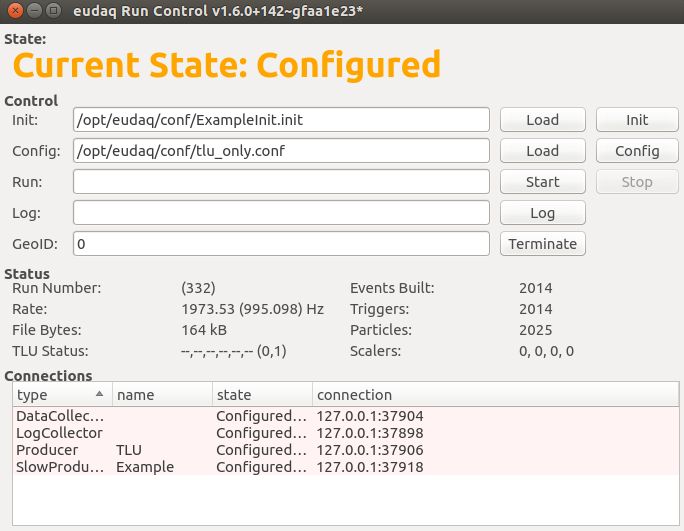
\includegraphics[width=0.6\textwidth]{src/images/RunControl}
    \caption{The Run Control graphical user interface.}
    \label{fig:RunControl}
  \end{center}
\end{figure}

Usually, no command-line option should be needed. 
If needed, it can be told to listen on a specific port (e.g. to run two copies on the same machine) 
using the \texttt{-a \param{port}} option, for example:
\begin{listing}[mybash]
$[./euRun.exe]$ -a 60000
\end{listing}
Note: If two copies of EUDAQ should run simultaneously,
the ports of the Log and DataCollectors have to be different!

\subsubsection{Log Collector}
It is recommended to start the Log Collector directly after having started the Run Control and before starting other processors in order to collect all log messages generated by all other processes.

\begin{figure}[htb]
  \begin{center}
    \includegraphics[width=\textwidth]{src/images/LogCollector}
    \caption{The Log Collector graphical user interface.}
    \label{fig:LogCollector}
  \end{center}
\end{figure}

Like the Run Control, there are also two versions of the Log Collector.
The graphical version is called \texttt{euLog.exe}, or \texttt{euLog.app} on Mac OS X,
and the text-based version is called \texttt{TestLogCollector.exe}.

If it is running on the same machine as the Run Control, it should not need any command-line options.
However, if it is running on a different machine, it must be told on which machine the Run Control is running.
By using the \texttt{-r \param{hostname}} option, the Log Collector knows where to connect to the Run Control, for example the Run Control runs on a machine haveing a local IP 192.168.0.1 and listening on the port 40000 (as default):
\begin{listing}[mybash]
$[./euLog.exe]$ -r tcp://192.168.0.1:44000
\end{listing}
The port can also be set using the \texttt{-a \param{port}} option, similar to the Run Control.

\subsubsection{Data Collector}
The Data Collector is the process that collects all the raw data from the Producers,
merges all the connected incoming streams into a single data stream, and writes it to file.
There is only a text-based version called \texttt{TestDataCollector.exe}.
It is recommended to start the Data Collector directly after having started the Run Control and RunControl and before starting other processors.

Like the Log Collector, it should be told where to connect to the Run Control if it is not running on the same machine.
Accordingly, the \texttt{-r} and \texttt{-a} options can be used, for example:
\begin{listing}[mybash]
$[./TestDataCollector.exe]$ -r tcp://192.168.0.1:44000
\end{listing}

It is also possible to run multiple Data Collector instances within
one EUDAQ session. 
This can be useful to reduce network traffic and
e.g. write the output of one producer to a locally attached disk. 
When running several Data Collectors simultaneously, the Run Control assigns a
Producer to a Data Collector by name: if the name of a Data Collector
matches that of a Producer, the latter will be given the address and
port of the former. 
There can be only one instance of an \emph{unnamed} Data
Collector which serves as the default for any non-matching Producer;
if no unnamed Data Collector is present, the first one connecting will
serve as the default.

The name of a Data Collector can be set with the
\texttt{-n} option, for example:
\begin{listing}[mybash]
$[./TestDataCollector.exe]$ -n myproducer
\end{listing}

If you wish to run several instances of the Data Collector on one
machine, you need to make sure that they listen to different addresses
using the \texttt{-a} option as described above. 
Furthermore, each Data Collector has to write to a different file by including the
\texttt{FilePattern} option in the corresponding section of your
configuration file (also see section \ref{sec:ConfigFiles}):

\begin{listing}[conf]
[DataCollector.myproducer]
FilePattern = "../data/run$6R_myproducer$X"
\end{listing}

\subsubsection{TLU Producer}
If you do not have a \gls{TLU} in your setup, you may skip this part.
Otherwise you should run a TLUProducer, which will configure the \gls{TLU},
and read out the timestamps and send them to the Data Collector.
On the computer with the \gls{TLU} connected, start the \texttt{TLUProducer.exe} program.
If this is not the same machine as the Run Control,
use the \texttt{-r} option as for the Data and Log Collectors, in this example:
\begin{listing}[mybash]
$[./TLUProducer.exe]$ -r 192.168.0.1:44000
\end{listing}
If the TLUProducer fails to start, make sure the permissions are set up correctly (see \autoref{sec:TLUperm}).

\subsubsection{NI Producer (Mimosa 26 sensors)}

\subsubsection{Online Monitor}
The Online Monitor reads the data file written by the Data Collector,
and generates several ROOT histograms that can be useful for online monitoring.
Since it reads the native data file directly (by using the corresponding DataConverterPlugin), it must be run on the same machine as the Data Collector.

\begin{figure}[htb]
  \begin{center}
    \includegraphics[width=0.8\textwidth]{src/images/OnlineMonCorrelations}
    \caption{The OnlineMon showing correlation plots between different
      Mimosa26 planes of the EUDET telescope.}
    \label{fig:OnlineMonPlots}
  \end{center}
\end{figure}

The Online Monitor can be run in one of two modes: online or offline.
In online mode, it connects to the Run Control, so it will know when new runs are started,
and it will automatically open each new data file as it is created.
To run it in online mode, the \texttt{-r} option may be used to assign Run Control, in this example:
\begin{listing}[mybash]
$[./OnlineMon.exe]$ -r 192.168.0.1:44000
\end{listing}
Note: The Online Monitor is working properly on Unix machines. In addition, it is recommended to run the Online Monitor on the same machine as the Data Collector.

In offline mode, there is no Run Control,
and it only analyses the data file it is given on the command line usind the \texttt{-f} option. 
An example command line is:
\begin{listing}[mybash]
$[./OnlineMon.exe]$ -f 5432
\end{listing}
This will run it in offline mode, opening the file corresponding to run 5432
(alternatively, the full path to a file may be given).

\subsubsection{TestProducer}
For testing purposes, you may use the Test Producer.
This works similarly to a real producer, but does not talk to any real hardware,
instead providing a menu for the user to manually send events
(or see the ExampleProducer, below).

\subsubsection{ExampleProducer}
The ExampleProducer was written to illustrate the writing of a new Producer (see \autoref{sec:Producers}).
However, it will actually generate some example data, and so can also be used for testing purposes.
It works more like a real Producer than the TestProducer,
in that it does not require user intervention to generate each trigger,
and the data generated emulates a simple (but realistic) sensor,
and can be properly converted, and therefore displayed in the Monitor.

\subsubsection{Other Producer(s)}
If you have a producer for your own hardware (see \autoref{sec:Producers}),
it should also have an option to set the address of the Run Control.

\subsubsection{Python Interface and Wrapper for Core EUDAQ Components}
\label{sssec:pywrapper}
A Python interface is provided for selected EUDAQ components:
RunControl, DataCollector and a Producer, that can be extended on the
Python side. The interface is realized through the \texttt{ctypes}
package that is part of every standard Python installation and
requires the \texttt{numpy} Python package to be installed. The
interface code for all components is located in the
\texttt{main/python} directory.

To use the interface and access the components as Python objects, the
wrapper must be loaded inside your Python script:

\begin{listing}[python]
  #!/usr/bin/env python2 
  execfile('PyEUDAQWrapper.py') # load ctypes wrapper

  prc = PyRunControl() # start run control with default settings
  # wait for more than one active connection to appear
  while prc.NumConnections < 2:
      sleep(1)
  prc.Configure("ExampleConfig") # load configuration file
  while not prc.AllOk:
      sleep(1) # sleep while waiting for all connected producers
  prc.StartRun()
\end{listing}

This little scripts creates a RunControl instance, sends a
configuration to all connected producers, waits for their reply, and
starts a new run. Several more extensive examples for using Python
with EUDAQ are located in the \texttt{python} directory in the main
EUDAQ directory.


\subsection{Running the DAQ}
To start the DAQ, all the necessary processes must be started in the correct order.
The first process must be the Run Control,
since all other processes will attempt to connect to it when they start up.
Then it is recommended to start the Log Collector,
since any log messages it receives may be useful
to help with debugging in case everything does not start as expected.
Next, the Data Collector should be started.
Finally all the Producers, and if needed, the RootMonitor.

\subsubsection{STARTRUN}\label{sec:STARTRUN}
The \texttt{STARTRUN} file, in the main \texttt{eudaq} directory
(as opposed to the \texttt{bin} subdirectory where the executables exist),
is a shell script that can be customized to load the appropriate processes for running the DAQ.
This allows you to start all the processes necessary with a single command.
If starting processes on other computers via SSH,
it is recommended to set up SSH keys so that the processes may be started without having to type a password.

In the future the \texttt{STARTRUN} script may be replaced with a more intelligent version
that uses a configuration file generated by the config script to decide what to load.

\subsubsection{Controlling the DAQ}
Once all the processes have been started, the DAQ can be configured, and runs may be started and stopped
using the Run Control (see \autoref{fig:RunControl}).

First the appropriate configuration should be selected from the drop-down list
(see \autoref{sec:ConfigFiles} for creating and editing configurations),
and the \texttt{GeoID} should be verified (see \autoref{sec:GeoID}), before continuing.

Then the \texttt{Config} button can be pressed,
which will send a configuration command
(with the contents of the selected configuration file) to all connected processes.
The full contents of the configuration file will also be stored
in the \gls{BORE} of the data file,
so that this information is always available along with the data.

Once all connected processes are fully configured, a run may be started, by pressing the \texttt{Start} button.
Whatever text is in the corresponding text box when the button is pressed
will be stored as a comment in the data file.
This can be used to help identify the different runs later.

Once a run is completed, it may be stopped by pressing the \texttt{Stop} button.
Runs will also stop and restart automatically when the data file reaches a threshold in size
(by default this is 1~GB).
This is because there is a file size limit of 2~GB for storage on the GRID,
and the processed files can grow bigger than the original native files.
The threshold size for restarting a run may be configured in the config file (see \autoref{sec:ConfigFiles}).

At any point a message may be sent to the log file by filling in the \texttt{Log} text box and pressing the corresponding button.
The text should appear in the LogCollector window, and will be stored in the log file for later access.

Once the run is stopped, the system may be reconfigured with a different configuration, or another run may be started.

\subsubsection{Config Files}\label{sec:ConfigFiles}
The \texttt{Config} drop-down in the Run Control is populated from the files in the \texttt{config} subdirectory.
These are just text files in a specific format, containing name-value pairs separated into different sections.
See \autoref{sec:ExampleConfig} for an example file.

Any text from a \texttt{\#} character until the end of the line is treated as a comment, and
ignored.  Each section in the config file is delimited by a name in square brackets
(e.g. \verb@[RunControl]@).  The name represents the type of process to which it applies; if there
are several such processes, then they can be differentiated by including the name after a period
(e.g. \verb@[Producer.Example]@).  Within each section, any number of parameters may be specified,
in the form \mbox{\texttt{Name = Value}}.  It is then up to the individual processes how these
parameters are interpreted.

The entire contents of the config file will be sent to all processes during the configuration, and
each process will have the appropriate section selected.  The file will also be attached to the
\gls{BORE}, so that it is available with the data later, even if the original config file is
modified or deleted.

\subsubsection{GeoID}\label{sec:GeoID}
The GeoID is a number representing the physical positioning of the telescope and DUT(s).
Each time a change is made to the telescope layout, this number should be incremented.
To change the number, double-click on it, and a window will appear with the new value.
By default it will increment the old value by one, so normally you should just click \texttt{OK},
but if necessary you may edit the value first.

The GeoID is inserted into the config file when it is sent, so it is also stored in the data file,
and will be used to select the correct GEAR file for alignment during the data analysis stage.

\subsection{Other Utilities}
There are a number of other utilities available that are not needed for running the DAQ,
but can be useful for other tasks such as debugging.
The executables are all located in the \texttt{bin} subdirectory.
They should all accept a help (\texttt{-h} or \texttt{--help}) option,
to print a summary of the available options.

\subsubsection{TLUControl}
The \texttt{TLUControl.exe} program is a standalone program for running the TLU without using the
full DAQ. The most commonly used parameters are shown below. For each option, the short (preceeded
by one dash) and the long (preceeded by two dashes) option names are shown (only one of the two
forms should be used for each option, but long and short options can be mixed together on the
command line), along with any parameters and their default value that will be used if the option is
not specified.

\begin{description}
\ttitem{-d --dutmask \param{mask = 0}}
The DUT mask; this defines which DUT connections are activated.  It is a bit-mask, so 1 means
connector 0, 2 means connector 1, etc..

\ttitem{-a --andmask \param{mask = 255}}
The AND mask; this defines which external trigger inputs are activated. It is a bit-mask, so 1
means channel 0, 2 means channel 1, etc.. The specified channels are ANDed together, and used to
generate a trigger signal.

\ttitem{-t --trigger \param{msecs = 0}}
Internal trigger period.  If non-zero, the \gls{TLU} will generate internal triggers with the
specified period in milliseconds. If set to zero, the internal trigger is off.

\ttitem{-i --dutinputs \param{values = ""}}
Input mode select. A sequence of comma-separated strings specifying which connectors to use for the
DUT inputs. Valid values are \texttt{RJ45}, \texttt{LEMO}, \texttt{HDMI}, and \texttt{NONE}.

\ttitem{-u --wait-for-user}
Pause the program after the \gls{TLU} is configured, before starting triggers. The default is to not
wait for the user.
\end{description}

Other parameters available are as follows:

\begin{description}
\ttitem{-o --ormask \param{mask = 0}}
The OR mask; this defines which external trigger inputs are activated. It is a bit-mask, so 1
means channel 0, 2 means channel 1, etc.. The specified channels are ORed together, and used to
generate a trigger signal.

\ttitem{-v --vetomask \param{mask = 0}}
The VETO mask; this defines which external trigger inputs are activated. It is a bit-mask, so 1
means channel 0, 2 means channel 1, etc.. The specified channels are used to veto the generation
of a trigger if they are active.

\ttitem{-w --wait \param{ms = 1000}}
Wait time. This is the time to wait between updates.

\ttitem{-n --notimestamp}
Indicates that the timestamp buffer should not be read out.

\ttitem{-q --quit}
Quit the program after configuring the TLU.

\ttitem{-s --save-file \param{filename = ""}}
     The filename to save trigger numbers and timestamps

\ttitem{-p --strobeperiod \param{cycles = 1000}}
Period for timing strobe (in \gls{TLU} clock cycles).

\ttitem{-l --strobelength \param{cycles = 100}}
Length of `on' time for timing strobe (in \gls{TLU} clock cycles).

\ttitem{-b --dutveto \param{mask = 0}}
Mask for enabling veto of triggers (`backpressure') by rasing DUT\_CLK.

\ttitem{-hm --handshakemode \param{nohandshake = 0}}
In this mode the TLU issues a fixed-length pulse on the trigger line (0 = no handshake).

\ttitem{-pw --powervctrl \param{mV = 800}}
[obsolete but provided for backward compatibility, please use \texttt{-pv}] Sets the Vcntl control
voltage to all PMTs. The range of values is between 0 and 1000 (or 0 and 2000 if the \gls{TLU} has
been modified by cutting \texttt{LC1} and jumpering \texttt{LO1} on the PMT Supply Daughterboard and
specifying the \texttt{-pm 1} option).

\ttitem{-pv --pmtvcntl \param{mV = 800}}
Sets the Vcntl control voltage to all PMTs (see option \texttt{-pw} for more details). Will override
the value of \texttt{-pw} if it is specified. If neither \texttt{-pw} or \texttt{-pv} is specified,
the default value will be used (and can be overridden on an individual PMT basis).

\ttitem{-p1 --pmtvcntl1 \param{mV}}
Sets the PMT Vcntl voltage for PMT1 (Chan 0) only. If not specified, the default or values specified
by \texttt{-pw} or \texttt{-pv} (which will override \texttt{-pw}) is used.

\ttitem{-p2 --pmtvcntl2 \param{mV}}
Sets the PMT Vcntl voltage for PMT2 (Chan 1) only. If not specified, the default or values specified
by \texttt{-pw} or \texttt{-pv} (which will override \texttt{-pw}) is used.

\ttitem{-p3 --pmtvcntl3 \param{mV}}
Sets the PMT Vcntl voltage for PMT3 (Chan 2) only. If not specified, the default or values specified
by \texttt{-pw} or \texttt{-pv} (which will override \texttt{-pw}) is used.

\ttitem{-p4 --pmtvcntl4 \param{mV}}
Sets the PMT Vcntl voltage for PMT4 (Chan 3) only. If not specified, the default or values specified
by \texttt{-pw} or \texttt{-pv} (which will override \texttt{-pw}) is used.

\ttitem{-pm --pmtvcntlmod \param{value = 0}}
Specifies whether the TLU PMT Supply Daughtercard is modified (\texttt{LC1} cut and \texttt{LO1}
jumpered) or not.  A \param{value} of 0 specifies that it is unmodified (and thus the Vcntl range is
from 0mV to 1000mV), and a \param{value} of 1 specifies that the \gls{TLU} is modified (and thus the
Vcntl range is from 0mV to 2000mV).  This feature is to accomodate newer Hamamatsu PMT models
(e.g. H10721) that require a control voltage range of, for instance, 500mV to 1100mV that are being
used in place of the older (discontinued, but what the \gls{TLU} was designed to accomodate and
control) models that required a control voltage of between 250mV and 900mV.

\ttitem{-f --bitfile \param{filename = ""}}
The bitfile containing the TLU firmware to be loaded.

\ttitem{-e --error-handler \param{value = 2}}
Error handler setting. Setting to 0 indicates the program should abort on an error. Setting it to a
value greater than 0 indicates the number of tries that should be attempted before generating an
exception.

\ttitem{-r --fwversion \param{value = 0}}
Specifies the firmware version to load (setting to 0 indicates the version should be chosen automatically).

\ttitem{-z --trace-file \param{filename = ""}}
The filename to save a trace of all USB accesses. Prepend a dash (`\texttt{-}') to output errors
only, or a plus (`\texttt{+}') for all data (including block transfers).
\end{description}

An example use of the command is shown below:

\begin{listing}[mybash]
$[./TLUControl.exe]$ -t 200 -d 3 -i LEMO,RJ45 -u
Using options:
TLU version = 0 (auto)
Bit file name = '' (auto)
Trigger interval = 200 ms (5 Hz)
DUT Mask  = 0x03 (3)
Veto Mask = 0x00 (0)
And Mask  = 0xff (255)
Or Mask   = 0x00 (0)
DUT inputs = LEMO,RJ45
Strobe period = 0x0003e8 (1000)
Strobe length = 0x000064 (100)
Enable DUT Veto = 0x00 (0)
Save file = '' (none)

TLU Version = v0.2c
TLU Serial number = 0x062b (1579)
Firmware file = TLU2_Toplevel.bit
Firmware version = 65
Library version = 65

Press enter to start triggers.

TLU Started!

Status:    20,00,--,--,--,-- (0,0)
Scalers:   0, 0, 0, 0
Particles: 2
Triggers:  0
Entries:   0
TS errors: 0, 0 (redundancy, re-read)
Timestamp: 0x8d768 (579432) = 0.00150891
Time: 0.009 s, Freq: 0 Hz, Average: 0 Hz

        0, 0x27fb479 (41923705) = 0.109174, diff=41923705
        1, 0x7139ab9 (118725305) = 0.309174, diff=76801600
        2, 0xba780f9 (195526905) = 0.509174, diff=76801600
        3, 0x103b6739 (272328505) = 0.709174, diff=76801600
        4, 0x14cf4d79 (349130105) = 0.909174, diff=76801600
Status:    20,00,--,--,--,-- (0,1)
Scalers:   0, 0, 0, 0
Particles: 7
Triggers:  5
Entries:   5
TS errors: 0, 0 (redundancy, re-read)
Timestamp: 0x1726fa48 (388430408) = 1.01152
Time: 1.023 s, Freq: 4.92913 Hz, Average: 4.88442 Hz

        5, 0x196333b9 (425931705) = 1.10917, diff=76801600
        6, 0x1df719f9 (502733305) = 1.30917, diff=76801600
        7, 0x228b0039 (579534905) = 1.50917, diff=76801600
        8, 0x271ee679 (656336505) = 1.70917, diff=76801600
        9, 0x2bb2ccb9 (733138105) = 1.90917, diff=76801600
Status:    20,00,--,--,--,-- (0,1)
Scalers:   0, 0, 0, 0
Particles: 12
Triggers:  10
Entries:   5
TS errors: 0, 0 (redundancy, re-read)
Timestamp: 0x2e5bb708 (777762568) = 2.02538
Time: 2.037 s, Freq: 4.93259 Hz, Average: 4.90838 Hz
^CQuitting...
\end{listing}

This sets up internal triggers at 5~Hz (200~ms period), and activates DUT inputs 0 and 1.
Input 0 is configured to use the LEMO connector, and input 1 to use the RJ45 connector.
The first part of the output just summarizes the input parameters.
The next part shows information about the version numbers of the TLU and the firmware.

It will then configure the \gls{TLU}, and if the \texttt{-u} option is used,
it will wait for the user to press enter before continuing.
The triggers are then enabled, and a summary of the status is printed out periodically
(by default every 1~second).
The program can be stopped cleanly by pressing \texttt{Ctrl-C}.

Each block of status output consists of:
\begin{myitemize}
\item a list of triggers, if there were any since the last update (the first time there are none),
each showing:
  \begin{myitemize}
  \item the trigger number,
  \item the timestamp of the trigger, in hex, decimal and converted to seconds,
  \item the difference since the last trigger.
  \end{myitemize}
\item the status of the \gls{DUT} connections (see below),
\item the values of the scalers on the external trigger inputs,
\item the number of ``particles'', which means all the potential triggers (including those that were vetoed),
\item the number of triggers that actually got sent to the \glspl{DUT},
\item the number of entries in the trigger buffer,
this should be equal to the number of triggers printed out at the top of the status block,
\item the number of timestamp errors detected by redundancy, and by re-reading,
\item the current timestamp value,
\item the time since the run started, the current trigger frequency, and the average frequency over the whole run.
\end{myitemize}

In the example output this block is repeated three times, before \texttt{Ctrl-C} is pressed to stop it.
The status is of the \gls{DUT} connections formatted as:
\begin{myitemize}
\item two digits for each \gls{DUT} connection consisting of:
  \begin{myitemize}
  \item two hyphens (\texttt{--}) if the connection is inactive, else
  \item the first digit represents the inputs from the \gls{DUT}; with the busy line in bit 0 and the clock line in bit 1
  (note the clock input can float low or high if a LEMO input is selected, as it is not connected),
  \item the second digit represents the state of the FSM, as defined in the \gls{TLU} manual\cite{Cussans2009}
  (0 is ready, 1 is waiting for busy high, 4 is waiting for busy low, 5 is \gls{DUT}-initiated veto, and F is an error condition).
  \end{myitemize}
\item then in parentheses:
  \begin{myitemize}
  \item the veto state (software veto in bit 0, overall veto in bit 1),
  \item the DMA state (1 when a DMA transfer is taking place).
  \end{myitemize}
\end{myitemize}

\subsubsection{VMETest}
The VMETest.exe program uses the EUDAQ VME library to perform VME accesses.
It can be useful for determining whether a VME card is responding at a particular address.
The available options are:
\begin{description}
\ttitem{-b \param{address}}
The base address for the VME accesses.
This value will be added to the offsets specified in the commands to give the actual address used.

\ttitem{-s \param{bytes}}
Sets the window size in bytes.
This is the amount of memory that is mapped into the VME address space.
Any accesses outside this range will result in an access violation.

\ttitem{-a \param{bits}}
The address bus width in bits.
Valid values are 16, 24, 32 or 64.

\ttitem{-d \param{bits}}
The data bus width in bits.
Valid values are 8, 16, 32 or 64.

\ttitem{-m \param{mode}}
The VME access mode.
Valid values are S (single accesses), B (BLT), M (MBLT), 2 (2eVME), E (2eSST) and T (2eSSTB).

\end{description}

The options set up the mode for the VME accesses.
Following the options, a number of commands can be specified to perform actual reads or writes.
The commands can be any of the following:
\begin{description}
\ttitem{r\param{offset}}
Reads a value from the specified offset, and displays the value read.

\ttitem{R\param{offset},\param{words}}
Performs a block read of the specified number of words, starting from the specified offset.

\ttitem{w\param{offset},\param{value}}
Writes the specified value to the specified offset.

\ttitem{W\param{offset},\param{value1}{[},\param{value2}\ldots{]}}
Performs a block write of the specified values, starting at the specified offset.

\end{description}

Numerical arguments to either the options or the commands can be given either in decimal,
or in hexadecimal by prefixing them with \texttt{0x}, as in C or C++.
Note that the options require a space between the option character and its argument,
but the commands must not have a space.
For example:

\begin{listing}[mybash]
$[./VMETest.exe]$ -b 0x180000 -a 24 -d 16 w0x20,123 r0x10
\end{listing}

This sets up a window starting at 180000 hex, in A24 address space with D16.
It then writes the value 123 to offset 32 (20 hex), and then reads the value at offset 16 (10 hex).

\subsubsection{TestReader}\label{sec:TestReader}
The \texttt{TestReader.exe} program will read a native data file,
and can display various pieces of information from the file.
Commonly used options are:
\begin{description}
\ttitem{-b}
Display the \gls{BORE}.

\ttitem{-e}
Display the \gls{EORE}.

\ttitem{-d \param{range}}
Display the specified range of event numbers.

\ttitem{-p}
Process the displayed events and display the corresponding StandardEvents.

\ttitem{-u}
Dump the raw data for the displayed events.

\ttitem{-s}
Try to resynchronize events based on the \gls{TLU} event number.
A full description of this option is outside the scope of this manual
(but if you don't know what it is, you probably don't need it).

\end{description}

After the options a list of one or more filenames can be given.
Any filenames that consist only of numerical digits
will be interpreted according to the input pattern
(by default this is ``\texttt{../data/run\$6R.raw}'',
where \texttt{\$6R} will be replaced with the run number padded to 6 digits).
For example:
\begin{listing}[mybash]
$[./TestReader.exe]$ -b -e -p -d 1-10,100,1000 example.raw 5432
\end{listing}

This will display the \gls{BORE} and \gls{EORE}, and the events 1 to 10, 100 and 1000,
processing them to also display the StandardEvents,
from the files \texttt{example.raw} and \texttt{../data/run005432.raw}.

\subsubsection{Converter}\label{sec:Converter}
The \texttt{Converter.exe} program will read a native data file,
optionally select just a subset of events from the file,
and can then write it out to another file in either the same native format, or a different format.
The most commonly used options are:
\begin{description}
\ttitem{-t \param{type}}
The file type to write out.
The available types are listed below.

\ttitem{-e \param{range}}
Select the specified range of event numbers.

\ttitem{-s}
Try to resynchronize events based on the TLU event number
(see TestReader in \autoref{sec:TestReader}).

\end{description}

The available output file types are as follows:

\begin{description}\phantomsection\label{lst:FileTypes}

\ttitem{native}
The native EUDAQ binary file format, consisting of a serialised stream of
\texttt{DetectorEvent}s, containing the raw data read out from the hardware.

\ttitem{standard}
Like the \texttt{native} format, this is also a serialised stream,
but in this case it contains \texttt{StandardEvent}s,
in which the raw data has been converted into a standard format.

\ttitem{lcio}
The standard \gls{LCIO} file format used by the analysis software.
This type is only available if EUDAQ was compiled with \gls{LCIO} support.

\ttitem{root}
A Root file containing a TTree with the hit pixel information.

\ttitem{text}
A simple text based format (not yet implemented).

\ttitem{mimoloop}
A text based format mimicking the output of the mimoloop program
(from Angelo Cotta Ramusino and Lorenzo Chiarelli at INFN Ferrara).

\end{description}

Although this program can be used to convert a native data file into \gls{LCIO} format,
the more usual (and therefore better tested) way is to use the EUTelescope converter.

\subsubsection{ClusterExtractor}
This program can be used to quickly extract some clusters from raw data.
It is not as sophisticated as the EUTelescope package, which should be preferred for real analysis,
but it can be useful for doing quick checks.
It will read a native data file, perform a basic clustering,
and then write these clusters to one text file per sensor plane.
The most commonly used options are:
\begin{description}
\ttitem{-p \param{pixels}}
The cluster size in pixels.
It should be an odd number, with 1 meaning no clustering (just pixels over threshold),
3 meaning 3\x{}3 pixel clusters, etc.

\ttitem{-n \param{adcs}}
The noise level (sigma) in ADC units.
This is used to scale the thresholds in terms of the noise.

\ttitem{-s \param{thresh}}
The threshold for seed pixels, in terms of the noise.

\ttitem{-c \param{thresh}}
The threshold for the total charge of a cluster,
in terms of the cumulative noise of all the pixels in the cluster.

\ttitem{-w}
Reports the cluster centre as the weighted average of the pixels,
instead of the position of the seed pixel.

\end{description}

An example use is:
\begin{listing}[mybash]
$[./ClusterExtractor.exe]$ -p 3 -n 3.5 -s 6 -c 10 -w 5432
\end{listing}

This will generate a number of text files named \texttt{runNNN\_eutel\_M.txt},
where \texttt{NNN} is the run number, and \texttt{M} is the sensor plane number.
The format of the output text files is as follows:
\begin{listing}[]
2       2       51487659237
 182    153     126
 241    120     125
3       1       51489095892
 111    67      346
5       1       51491334074
 113    141     171
7       2       51495330212
 252    240     305
 95     170     189
\end{listing}

The first line contains the event number,
the number of clusters, and the TLU timestamp.
Then for each cluster there is one line,
containing the \texttt{x} and \texttt{y} coordinates of the cluster centre,
and the total charge in ADC units.
The cluster lines are prepended with a space to make it easier to scan the file by eye.


\subsubsection{MagicLogBook}
This program is designed to extract as much information as possible from data files and log files,
in order to reconstruct a log book.
Despite its name, it is in fact not magical,
so it is preferable to keep a good log book during running,
rather than relying on this program to generate it later.

The available options are listed below:
\begin{description}
\ttitem{-f \param{fields}}
A list of fields to include in the output, in the form \texttt{name=value},
with multiple fields separated by commas.
If a predefined list is also specified these will be appended to the list.

\ttitem{-s \param{separator}}
The separator to use between fields in the output. The default is a tab character.

\ttitem{-h \param{string}}
A string that appears at the beginning of the header line (with the list of field names),
that can be used to differentiate it from the other lines. The default is an empty string.

\ttitem{-p {name}}
Use a predefined list of fields.
Currently available values are \texttt{normal} and \texttt{full}.

\ttitem{-o \param{file}}
The output filename. By default the standard output is used.

\end{description}

The easiest method of running is to use a predefined list of fields.
There are currently two predefined lists available: \texttt{normal} and \texttt{full}.
If neither of these are suitable, contact the EUDAQ maintainer,
as it may be possible to add more options.

The \texttt{normal} list includes:
\begin{myitemize}
  \item the run number,
  \item the config file name,
  \item the run start time,
  \item for the \glspl{EUDRB}:
  \begin{myitemize}
    \item the mode,
    \item the sensor type,
    \item whether they are running unsynchronized,
    \item the number of boards,
    \item and the firmware version.
  \end{myitemize}
  \item and for the \gls{TLU}:
    \begin{myitemize}
    \item the internal trigger interval,
    \item the AND mask,
    \item the DUT mask,
    \item and the firmware version.
  \end{myitemize}
\end{myitemize}

The \texttt{full} list includes all the values from the \texttt{normal} list,
plus the number of events in the run and the end of run time.
This is because these values can only be known by reading
the whole data file to the end, which is slow, especially for large data files.

If necessary, other information is available using custom fields,
although the syntax for these is a bit complicated,
since it is designed to be as flexible as possible at specifying any information in the data file.
In the future it may be redefined in order to simplify it if possible.
Therefore it is recommended to use a predefined list of fields where possible.
Custom fields are specified as a comma separated list of items in the form \texttt{name=value},
with the name being what will appear on the header line of the output,
and the value specifying what exactly to extract from the file.
The possible values are illustrated below, although not exhaustively:

\begin{mydescription}
  \ttitem{events$^\ast$} The number of events in the run.
  \ttitem{config} The configuration name, or:
  \begin{mydescription}
    \ttitem{config:section:key} The value of the \texttt{key} from the corresponding \texttt{section} in the config
    (e.g. \texttt{config:Producer.EUDRB:NumBoards}).
  \end{mydescription}
  \item{\texttt{bore}, \texttt{tlu}, \texttt{eudrb}, \texttt{eore}$^\ast$:} Something from the \gls{BORE},
  the \texttt{TLUEvent} or \texttt{EUDRBEvent} subevents of the \gls{BORE}, or the \gls{EORE}, respectively:
  \begin{mydescription}
    \ttitem{bore:.Run} The run number
    \ttitem{bore:\param{name}} Otherwise, if the second part does not start with a period, the value of the tag \param{name} is used
    (e.g. \texttt{tlu:DutMask} or \texttt{eudrb:MODE}).
  \end{mydescription}
  \ttitem{log} Something from the log file (not implemented yet).
\end{mydescription}

$^\ast$ items marked with an asterisk require reading the whole data file, and are therefore slow,
especially when large data files are involved.

Note that the \texttt{EUDRBEvent} is now deprecated, having been replaced by the \texttt{RawDataEvent},
but there is currently no way to specify this.

The \texttt{MagicLogBook} command is used as follows:

\begin{listing}[mybash]
$[./MagicLogBook.exe]$ -p normal ../data/*.raw
\end{listing}

This will produce an output similar to the following:
\begin{listing}[]
Run  Config     Mode Det Start                   U P Trg AND  DUT  Tfw Efw
6371 eudet-beam          2009-07-29 07:44:39.535 1 6   0 0xf  0x10 241
6372 eudet-beam          2009-07-29 08:03:05.079 1 6   0 0xf  0x10 241
6373 eudet-m26test       2009-07-30 09:57:45.157 1 6 255 0xff 0x12 241
6374 eudet-m26test       2009-07-30 10:00:45.205 1 6 255 0xff 0x12 241
6375 eudet-m26test       2009-07-30 10:05:38.625 1 6   1 0xff 0x12 241
6376 eudet-m26test       2009-07-30 10:10:00.107 1 6   1 0xff 0x12 241
6379 eudet-m26test       2009-07-30 10:13:05.322 1 6   1 0xff 0x12 241
\end{listing}

Note that the header row has been modified slightly to fit into the page width:
the \texttt{U} should be \texttt{UnSync}, \texttt{P} should be \texttt{Planes},
\texttt{Trg} should be \texttt{TriggerInterval}, \texttt{Tfw} should be \texttt{TLUfw},
and \texttt{Efw} should be \texttt{EUDRBfw}.
The columns \texttt{Mode}, \texttt{Det} and \texttt{EUDRBfw} are missing from the output
due to the fact that this information is now stored in a \texttt{RawDataEvent},
which is not currently accessible with this version of the program.

\subsubsection{FileChecker}

This is a small utility that reads raw data files and checks if all events are
readable, can be syncronised using the TLU trigger id and lists which type
of subevents the file contains.

It should be called with list of file paths or run numbers. For any argument
that consist only of numerical digits the file path is constructed by
substituting \texttt{\$6R} in the input pattern (defaults to
``\texttt{../data/run\$6R.raw}'') with the run number padded to 6 digits.

For example:
\begin{listing}[mybash]
$[./FileChecker.exe]$ {6045..6050}
\end{listing}

This would produce the following output.
\begin{listing}[]
run     valid  num_events  contains                   errors                    
------  -----  ----------  -------------------------  ----------------------
  6045   true       13131  MUPIX4,NI,TLU                                        
  6046   true           1  MUPIX4,NI,TLU                                        
  6047   true       14674  MUPIX4,NI,TLU                                        
  6048   true        7776  MUPIX4,NI,TLU                                        
  6049  false           0                             no events in the file.    
  6050  false          -1                             read error. 
\end{listing}

\subsubsection{Others}
Some programs that are less used (or recently added)
may not be described here.
If they look interesting, you can find out more about them
by running them with the help (\texttt{-h} or \texttt{--help}) option,
or by examining the source code.

% !TEX root = EUDAQUserManual.tex
\section{Writing a Producer}\label{sec:ProducerWriting}
Producers are the binding part between a user DAQ and the central EUDAQ Run Control. The base class of Producer is eudaq::Producer. The eudaq::Producer is an inherited class of eudaq::CommandReceiver which receives commands from the eudaq::RunControl. It also maintains a set of eudaq::DataSender comamnds which allow binary data (eudaq::Event) to be sent to each destination.\\

\subsection{Producer Prototype}\label{sec:Producer_hh}

\autoref{producerdef}, below, is part of the header file which declares the eudaq::Producer. You are required to write the user Producer derived from eudaq::Producer. According the the set of commands (\autoref{sec:command}) in the EUDAQ framework, there are six virtual functions which should be implemented in the user producer. They are DoInitialise(), DoConfigure(), DoStopRun(), DoStartRun(), DoReset() and DoTerminate(). These command-related functions should return as soon as possible since no further command can be execuseted until the current command is finished. \\

\lstinputlisting[label=producerdef, style=cpp, linerange=BEGINDECLEAR-ENDDECLEAR]{../../main/lib/core/include/eudaq/Producer.hh}

The virtual function Exec() can optionally be implemented in the user Producer. If this is not implemented, the default Exec() will connect to the RunControl and goes into an infinite loop and will only return when the Terminate command is executed. In case you are going to implement an Exec() function, please read the source code to find detailed information.

\subsection{Example Source Code: Dummy Event Producer}\label{sec:Ex0Producer_cc}
\subsubsection{Declaration}
Here we outline an example implementation of a user Producer. The full source code is available at file path user/example/module/src/Ex0Producer.cc. There are six command related functions, a constructor function and a \texttt{Mainloop} function in the declaration part: \\

\lstinputlisting[label=ls:ex0producerdef_declaration, style=cpp, linerange=BEG*DEC-END*DEC]{../../user/example/module/src/Ex0Producer.cc}

The line \lstinline[style=cpp]{static const uint32_t m_id_factory = eudaq::cstr2hash("Ex0Producer")}, defines a static number which is a hash from the name string. This number will be used later as a ID to register this \lstinline[style=cpp]{Ex0Producer} to the EUDAQ runtime environment.

\subsubsection{Register to Factory}
To make the EUDAQ framework know of the existence of \lstinline[style=cpp]{Ex0Producer}, this Producer should be registered to \lstinline[style=cpp]{eudaq::Factory<eudaq::Producer>} with its static ID number. The input parameter types of the constructor function are also provided to the Register function. See the example code:
\lstinputlisting[label=ls:ex0producerdef_factory, style=cpp, linerange=BEG*REG-END*REG]{../../user/example/module/src/Ex0Producer.cc}

\subsubsection{Constructor}
The Constructor function takes in two parameters, the runtime name of the instance of the Producer and the address of the RunControl. 
\lstinputlisting[style=cpp, linerange=BEG*CON-BEG*INI]{../../user/example/module/src/Ex0Producer.cc}
In this example of Ex0Producer, the constructor function does nothing beside passing parameters to the base constructor function of Producer and initializes the \lstinline[style=cpp]{m_exit_of_run} variable.

\subsubsection{DoInitialise}
This method is called whenever an initialize command is received from the RunControl. When this function is called, the correlated section of the initialization file have arrived to the Producer from the RunControl. This initialization section can be obtained by: \\
\lstinline[style=cpp]{eudaq::ConfigurationSPC eudaq::CommandReceiver::GetInitConfiguration()} \\

Here is an example \lstinline[style=cpp]{DoInitialise} of the Ex0Producer:
\lstinputlisting[style=cpp, linerange=BEG*INI-BEG*CONF]{../../user/example/module/src/Ex0Producer.cc}
The Configuration object \lstinline[style=cpp]{ini} is obtained. According to the value DUMMY\_STRING and DUMMY\_FILE\_PATH in \lstinline[style=cpp]{ini} object, a new file is opened and filled by dummy data. The path of the file is saved as a variable member for later access of this dummy data file.

\subsubsection{DoConfigure}
This method is called whenever a configure command is received from the RunControl. When this function is called, the correlated section of configuration file has arrived to the Producer from the RunControl. The configuration section named by the Producer runtime name can be obtained by:\\
\lstinline[style=cpp]{eudaq::ConfigurationSPC eudaq::CommandReceiver::GetConfiguration()} \\

Here is an example \lstinline[style=cpp]{DoConfigure} of Ex0Producer:
\lstinputlisting[style=cpp, linerange=BEG*CONF-BEG*RUN]{../../user/example/module/src/Ex0Producer.cc}
The variables \lstinline[style=cpp]{m_ms_busy}, \lstinline[style=cpp]{m_flag_ts} and \lstinline[style=cpp]{m_flag_tg} are set according to the Configuration object.

\subsubsection{DoStartRun}\label{sec:ex0prdstart}
This method is called whenever a StartRun command is received from the RunControl. When this function is called, the run-number has already been increased by 1. For a real hardware specific Producer, the hardware is told to startup.
Here is an example \lstinline[style=cpp]{DoStartRun} of Ex0Producer:
\lstinputlisting[style=cpp, linerange=BEG*RUN-BEG*STOP]{../../user/example/module/src/Ex0Producer.cc}
Instead of talking to real hardware, a file is opened. Then, a new thread is started using the function \lstinline[style=cpp]{Mainloop}.

\subsubsection{DoStopRun}
This method is called whenever a StopRun command is received from the RunControl. Here is an example \lstinline[style=cpp]{DoStopRun} of Ex0Producer:
\lstinputlisting[style=cpp, linerange=BEG*STOP-BEG*RST]{../../user/example/module/src/Ex0Producer.cc}

\subsubsection{DoReset}
When the Producer goes into an error state, only the Reset command is acceptable. It is recommended to reset all member variables to their original value when the producer object is instanced.\\
Here is an example \lstinline[style=cpp]{DoReset} of Ex0Producer: 
\lstinputlisting[style=cpp, linerange=BEG*RST-BEG*TER]{../../user/example/module/src/Ex0Producer.cc}
For any case the data thread is running, it should be stopped.

\subsubsection{DoTerminate}
This method is called whenever a StopRun command is received from the RunControl. After the return of \lstinline[style=cpp]{DoTerminate}, the application will exit.\\
Here is an example \lstinline[style=cpp]{DoStopRun} of Ex0Producer:
\lstinputlisting[style=cpp, linerange=BEG*TER-BEG*LOOP]{../../user/example/module/src/Ex0Producer.cc}
The data thread is then closed. 

\subsubsection{Send Event}
In \lstinline[style=cpp]{DoStartRun}, a data thread is created with the function \lstinline[style=cpp]{Mainloop}. Here is the implementation of this function. The generated data Event depends on the value set by \lstinline[style=cpp]{DoInitialise} and \lstinline[style=cpp]{DoConfigure}.
\lstinputlisting[style=cpp, linerange=BEG*LOOP-END*IMP]{../../user/example/module/src/Ex0Producer.cc}
In each loop, a new object of Event named Ex0Event is created. Trigger number and Timestamp are options to be set depending on the flags. A data block with 100 zeros is filled to the Event object by id 0. Another data block read from file is filled to some Event object by id 2. Then, this Event object is sent out by \lstinline[style=cpp]{SendEvent(std::move(ev))}. The first Event object has a flag BORE by the method \lstinline[style=cpp]{eudaq::Event::SetBORE()}

\paragraph{Tags}\label{sec:Tags}
The \texttt{Event} class also provide the option to store tags.
Tags are name-value pairs containing additional information which does not qualify as regular DAQ data which is written in the binary blocks.
Particularly in the \gls{BORE} this is very useful to store information about the exact sensor configuration which might be required in order to be able to decode the raw data stored.
A tag is stored as follows:
\begin{listing}
event.SetTag("Temperature", 42);
\end{listing}

The value corresponding to the tag can be set as an arbitrary type (in this case an integer),
it will be converted to a STL string internally.

\subsubsection{Error}\label{sec:Error}
In the case when the Producer fails to run a command function an exception like this will be produced \\
\lstinline[style=cpp]{EUDAQ_THROW("dummy data file (" + m_dummy_data_path +") can not open for writing")}\\
An error message is then sent to the RunControl.



% !TEX root = EUDAQUserManual.tex
\section{Data Conversion}
Data are stored on disk, by default, in a native binary format, containing the raw data as read out by the various Producers.
It is the same format used for serialising the data over the socket connection to the Data Collector.
To be legible to other software components, this data must be converted into a standardised format so that the monitoring and analysis software
does not require specific information about the functionalities and data encoding scheme of every detector, but can be applied generically to any sensor.

Currently, two different formats are provided for this purpose.
The first is the \texttt{StandardEvent} type, an EUDAQ-internal class used by the online monitoring tool and other utilities of the framework. It is a very simplified format tailored towards pixelated tracking detectors.
The second type is the \gls{LCIO} standard format from the linear collider community,
which is also used by the EUTelescope analysis software.


\subsection{StandardEvent and StandardPlane}
The \texttt{StandardEvent} is a class designed to represent pixel sensor data in a reasonably easy to use way,
but still be flexible enough to store the data from a wide range of different sensors.

Each \texttt{StandardEvent} represents one event of data from the whole telescope and any \glspl{DUT},
so a run will consist of a sequence of \texttt{StandardEvent}s.
It inherits from the \texttt{Event} base class, meaning that it has a run number, an event number, an optional timestamp,
and may also contain tags (see \autoref{sec:Tags}).

The decoded pixel data is stored in an array of \texttt{StandardPlane}s, each representing one sensor plane of the telescope or \gls{DUT}.
Each \texttt{StandardPlane} contains the charge values from the pixels of one sensor,
and may contain several frames in cases where the sensor is read out multiple times per event.
It also has the concept of a ``result'' frame, which is calculated from the one or more of the source frames
according to different rules that may be specified with flags.
The result frame contains only one charge value per pixel, with a positive signal,
and is what will be used for the analysis.
It may consist of either differences between the original frames (e.g. in the case of \gls{CDS}),
a sum of all original frames, or specific parts of the different frames selected according to the pivot information.
Flags may be set to select which of the different methods is used.
It may also contain a submatrix number per pixel, which can be used to differentiate different parts of the sensor,
so that they may be analyzed separately later, and a pivot boolean (true or false) per pixel,
which can be used to indicate whether the pixel was sampled before or after the trigger,
and is used to determine which parts of the sensor to combine when the \texttt{FLAG\_NEEDCDS} flag is set.

Both the \texttt{StandardEvent} and the \texttt{StandardPlane} classes are defined in the following header file:
\begin{listing}
#include "eudaq/StandardEvent.hh"
\end{listing}

In general, a user should not need to construct a \texttt{StandardEvent} object,
but should create one or more \texttt{StandardPlane}s, that will be added to a given \texttt{StandardEvent}.

\subsubsection{Constructor}
The \texttt{StandardPlane} constructor has the following signature:
\begin{listing}
StandardPlane(unsigned id, const std::string & type,
              const std::string & sensor = "");
\end{listing}

Where \texttt{id} is an arbitrary numerical identifier for the plane
that can be used to differentiate between different planes of the same type,
\texttt{type} is the type of the Producer that generated the frame
(should be the same as that in the \texttt{Producer} and the \texttt{DataConverterPlugin}),
and \texttt{sensor} is the name of the sensor,
in the case that the Producer can read out more than one type of sensor.

\subsubsection{SetSizeRaw and SetSizeZS}
Once a \texttt{StandardPlane} has been constructed, the size should be set.
There are two methods for doing this,
depending on whether the data are stored in raw or zero-suppressed mode.
In raw mode all pixels are stored, whether they have a signal or not.
In zero-suppressed mode, only those with a signal above a certain threshold are stored,
along with their coordinates, and any below the threshold are suppressed.

The signature of the \texttt{SetSizeRaw} method is:
\begin{listing}
void SetSizeRaw(unsigned w, unsigned h, unsigned frames = 1, int flags = 0);
\end{listing}

Where \texttt{w} is the full width of the sensor (in the x-direction, usually columns) in pixels,
h is the full height of the sensor (in the y-direction, usually rows) in pixels, \texttt{frames} is the number of frames,
and \texttt{flags} may be a combination of the following values, separated by a bitwise OR (i.e. \texttt{|}):

\begin{description}
\ttitem{FLAG\_NEEDCDS} Indicates that the data are in 2 or 3 frames
and that neighbouring frames should be subtracted to produce the result.

\ttitem{FLAG\_NEGATIVE} Indicates that the charge values are negative,
so should be negated to produce the result.

\ttitem{FLAG\_ACCUMULATE} Indicates that all frames should be summed to produce the result.

\ttitem{FLAG\_WITHPIVOT} Indicates that pivot information is stored per pixel,
and should be used for constructing the result.

\ttitem{FLAG\_WITHSUBMAT} Indicates that submatrix information is stored per pixel.

\ttitem{FLAG\_DIFFCOORDS} Indicates that each frame can have different coordinates,
in the case of zero-suppressed data, otherwise all frames will share the same coordinates.

\end{description}

The signature of the \texttt{SetSizeZS} method is a follows:
\begin{listing}
void SetSizeZS(unsigned w, unsigned h, unsigned npix,
               unsigned frames = 1, int flags = 0);
\end{listing}

Where all parameters are the same as in \texttt{SetSizeRaw}, but there is an extra parameter (\texttt{npix})
that specifies how many pixels to preallocate.
If the number of pixels above threshold is known, this may be used to allocate them all at once.
If not, then this parameter may be set to zero, and pixels can be allocated as needed
(but note that this way may be slower, since memory will need to be reallocated for each new pixel).

\subsubsection{SetPixel and PushPixel}
Once the size has been set, the values of the pixels can then be loaded into the \texttt{StandardPlane}.
There are two methods for doing this: \texttt{SetPixel}, that sets the value of an already allocated pixel,
and \texttt{PushPixel} that allocates space for a new pixel and sets that.

The signatures of \texttt{SetPixel} are as follows:
\begin{listing}
void SetPixel(unsigned index, unsigned x, unsigned y, unsigned pix,
              bool pivot = false, unsigned frame = 0);
void SetPixel(unsigned index, unsigned x, unsigned y, unsigned pix,
              unsigned frame);
\end{listing}

where \texttt{index} is the index of the pixel to set, \texttt{x} and \texttt{y} are the coordinates of the pixel,
and \texttt{pix} is the charge value for the pixel.
The value of the pivot, and the frame number may optionally be set also, if relevant.
Note that if only the pivot is set, care should be taken that it is of type \texttt{bool}
to avoid accidentally setting the frame instead.

The signatures of \texttt{PushPixel} are as follows:
\begin{listing}
void PushPixel(unsigned x, unsigned y, unsigned pix,
               bool pivot = false, unsigned frame = 0);
void PushPixel(unsigned x, unsigned y, unsigned pix,
               unsigned frame);
\end{listing}

where all parameters are the same as in \texttt{SetPixel}.
The only difference being the lack of an \texttt{index} parameter,
since this will always allocate a new pixel and append it to the existing list.

\subsubsection{Setting other information}
Other than the pixel values, the \texttt{StandardPlane} also stores some other information
that should be set if applicable:

\begin{listing}
void SetTLUEvent(unsigned ev);
\end{listing}

This sets the trigger ID as read out from the \gls{TLU}.
If it was read out and stored, it should be set using this method to allow cross checks in the analysis.

\begin{listing}
void SetPivotPixel(unsigned p);
\end{listing}

This sets the value of the pivot pixel (or pivot row etc. -- the value is arbitrary).
It is only here to allow cross-checks in the analysis;
if the pixels are to be combined using the pivot information,
then it should also be set in the per-pixel pivot values.
The value here cannot be used for that purpose since the order of reading out the pixels is not in general known.

\begin{listing}
void SetFlags(FLAGS flags);
\end{listing}

Some flags may be set after calling \texttt{SetSizeRaw} or \texttt{SetSizeZS}, but this is not possible with the flags
\texttt{FLAG\_WITHPIVOT}, \texttt{FLAG\_WITHSUBMAT} or \texttt{FLAG\_DIFFCOORDS} since these
flags affect how memory is allocated by those methods.

\subsubsection{Adding Planes to the StandardEvent}
Once the plane has been constructed and filled, it may be added to a \texttt{StandardPlane} using the following method:
\begin{listing}
StandardPlane & AddPlane(const StandardPlane &);
\end{listing}

This will copy the plane into the list of \texttt{StandardPlane}s stored by the \texttt{StandardEvent}.
It will return a reference to the copy of the plane, that can be used to make further modifications if necessary.

\subsubsection{Extracting information}
The \texttt{StandardEvent} inherits the following methods from the \texttt{Event} base class:
\begin{listing}
unsigned GetRunNumber() const;
unsigned GetEventNumber() const;
uint64_t GetTimestamp() const;
T GetTag(const std::string & name, T def) const;
\end{listing}

allowing access to the run number, event number, timestamp (if set) and any tags (where T is an arbitrary type).
It also has the following methods to access the \texttt{StandardPlane}s that it contains:
\begin{listing}
size_t NumPlanes() const;
const StandardPlane & GetPlane(size_t i) const;
\end{listing}

These return the number of planes stored, and a reference to a particular plane, respectively.
The individual planes can then be examined using the following methods:
\begin{listing}
const std::string & Type() const;
const std::string & Sensor() const;
unsigned ID() const;
unsigned TLUEvent() const;
unsigned PivotPixel() const;
\end{listing}

These return the type of the plane (i.e. the type of Producer / DataConverter that generated it),
the type of sensor for the plane (in the case that the plane type can hold different types of sensor data),
the ID of the plane (used to differentiate different planes of the same type),
the TLU trigger ID for the plane (if it was read out and stored)
and the value of the pivot pixel (or pivot row) for the plane.
Further information about the plane is available in:
\begin{listing}
unsigned XSize() const;
unsigned YSize() const;
unsigned NumFrames() const;
unsigned TotalPixels() const;
unsigned HitPixels() const;
unsigned HitPixels(unsigned frame) const;
\end{listing}

These return the full width and height of the sensor in pixels,
the number of frames stored for the plane,
total number of pixels for the plane (i.e. full width \x{} height),
the number of pixels over threshold (for zero-suppressed data) in the result frame,
and the number of pixels over threshold in a particular source frame.

Note that for the \texttt{HitPixels} method, there are two versions;
the first takes no parameter and returns the number of hit pixels in the result frame,
while the second takes the frame number as a parameter and returns the number of hit pixels
in that frame from the underlying source data.
Normally the first version would be used, unless access is needed to the raw data from the sensor.
Similarly, the other methods for accessing the data all have two versions:

\begin{listing}
double GetPixel(unsigned index) const;
double GetX(unsigned index) const;
double GetY(unsigned index) const;
const std::vector<pixel_t> & PixVector() const;
const std::vector<coord_t> & XVector() const;
const std::vector<coord_t> & YVector() const;
\end{listing}

These return the charge value, the x coordinate and the y coordinate of a particular pixel
(for the first three methods),
or a vector of these values for all pixels in the frame (for the final three methods.

Here, \texttt{coord\_t} and \texttt{pixel\_t} are both \texttt{double}, even though the values stored are usually integers.
This is in order to make the \texttt{StandardPlane} as general as possible, allowing it to store, for example,
clusters with non-integer coordinates instead of pixels, and it also makes it easier to pass the values directly
into Root histograms without first having to convert them to \texttt{double}.
All the above methods also have a version taking the frame number
(as the second parameter if they already have one parameter),
which returns the information from the underlying source frame instead of the result frame.

\subsection{LCIO and LCEvent}\label{sec:LCIO}
% TODO: describe LCIO format
Another option available with the framework is the ouput of data as \gls{LCIO} events.
The LCIO format is a very flexible container defined and used by the linear collider community. The exact encoding of the data relies upon the requirements from the user and cannot be described in a generic way.

Many tracking detectors rely on the additional classes provided by the EUTelescope data analysis framework, examples for implementations can be found in the respective converter plugins in the EUDAQ source tree.

\subsection{DataConverterPlugin}
In order to allow different \glspl{DUT} to easily incorporate their data into the monitoring and analysis chain,
the \texttt{DataConverterPlugin} system was developed.
This allows all the conversion code for each producer to be kept in one file,
with the necessary parts being called automatically as needed.
This section describes how to write a new converter plugin,
to use existing converter plugins see \autoref{sec:PluginManager}.

Writing a converter plugin for a new producer involves defining a new class
that derives from the \texttt{DataConverterPlugin} base class and implementing a few methods.
Each converter plugin contains a unique string that defines
which type of \texttt{RawDataEvent}s it is able to convert.
This is the same string that is set in the \texttt{RawDataEvent} when it is created by the relevant producer.
The \texttt{DataConverterPlugin} class is defined in the following header:
\begin{listing}
#include "eudaq/DataConverterPlugin.hh"
\end{listing}

The methods to be implemented are described below,
and a full example is provided in \autoref{sec:ExampleConverter}.

\subsubsection{Constructor}
The constructor should call the \texttt{DataConverterPlugin} constructor, and pass as a parameter the
string representing the type of \texttt{RawDataEvent} this plugin can convert.
A single static instance of the converter should then be defined,
and instantiated in the source file.
This is illustrated below:
\begin{listing}[C++]
class ExampleConverterPlugin : public eudaq::DataConverterPlugin {
  ExampleConverterPlugin() : eudaq::DataConverterPlugin("EXAMPLE") {
    // constructor...
  }
  // more methods...
  static ExampleConverterPlugin m_instance;
};
ExampleConverterPlugin ExampleConverterPlugin::m_instance;
\end{listing}

this will cause the constructor to be called during initialization of the program,
and the \texttt{DataConverterPlugin} constructor will automatically register the plugin
and make it available in the \texttt{PluginManager}.

\subsubsection{Initialization}
Every time a new run is started, the \texttt{Initialize} method will be called.
It has the following signature:
\begin{listing}
virtual void Initialize(const Event & ev, const Configuration & c);
\end{listing}

It receives as parameters the \gls{BORE}, and the configuration used for the run.
The plugin may extract any tags from the \gls{BORE}, or other information from the configuration,
and store it in member variables for use during decoding.

\subsubsection{GetTriggerID}
Since each producer that reads out the trigger ID from the \gls{TLU} stores it differently in the raw data,
there is no general way to extract this information.
The \texttt{GetTriggerID} method remedies this, by providing a generic interface to access the trigger ID.
The signature is as follows:
\begin{listing}
virtual unsigned GetTriggerID(const Event & ev) const;
\end{listing}

It receives the \texttt{Event} as a parameter, from which it should extract the \gls{TLU} trigger ID,
and return it as an unsigned integer.

\subsubsection{GetStandardEvent}
This method should extract the sensor data from the \texttt{RawDataEvent} input parameter,
and fill in the \texttt{StandardEvent} by adding the appropriate number of \texttt{StandardPlane}s
(one per sensor plane).
The method signature is:
\begin{listing}
virtual bool GetStandardSubEvent(StandardEvent & out,
                                 const Event & in) const;
\end{listing}

It should return \texttt{true} if it successfully updated the \texttt{StandardEvent}, or \texttt{false} to indicate an error.

\subsubsection{GetLCIOEvent}
Similar to \texttt{GetStandardEvent}, the \texttt{GetLCIOEvent} method converts a \texttt{RawDataEvent}
into a standardized format, in this case \gls{LCIO}.
The signature is:
\begin{listing}
virtual lcio::LCEvent * GetLCIOEvent(const Event * ev) const;
\end{listing}

It receives the \texttt{RawDataEvent} as a parameter, and should return a pointer to a new LCEvent
if the conversion is successful. In the event of an error, it should return a null pointer.

\include{src/OtherParts}
% !TEX root = EUDAQUserManual.tex
\section{Reporting Issues}
\label{sec:reporting}
The GitHub server, on which EUDAQ is hosted, provides a system for reporting bugs and for requesting new features.
It is accessible at the following address: 

\url{https://github.com/eudaq/eudaq/issues}.

Here you may submit new reports (you are required to register first to do this),
or follow the status of existing bugs and feature requests.
This is recommended over (or at least, as well as) sending an email to the developers,
as it ensures a record of the issue is available, and others may follow the progress.
%TODO: expand

% !TEX root = EUDAQUserManual.tex
\section{Developing and Contributing to EUDAQ}
\label{sec:contributing}

\subsection{Regression Testing}
\label{sec:ctest}

If a CMake version later than 2.8.0 is found and Python is installed
together with the \texttt{numpy} package, several regression tests are made
available that can be executed through CTest. The tests are based on
the Python wrapper around EUDAQ components as described in
section~\ref{sssec:pywrapper}. Run the tests by typing

\begin{listing}[mybash]
  cd build
  cmake ..
  ctest
\end{listing}

This starts the script \texttt{etc/tests/run\_dummydataproduction.py}
which runs a short DAQ session with instances of RunControl,
DataCollector and a (dummy) Producer and compares the output to a
reference file stored on AFS at DESY. If your system is set up
correctly, you have access to the reference file, and the basic
components of the EUDAQ library work, all tests should pass.
To see the output of failing tests, you can add the
\texttt{--output-on-failure} parameter to the CTest command.

These basic tests can easily be extended to test other parts of the
core framework or of your own producer. Take a look at the
\texttt{etc/tests/testing.cmake} CMake script and the central
\texttt{CMakeLists.txt} file where it is included for an example of
how to set up tests with CTest.

The automated nightly tests are defined in CMake scripts located in
\texttt{etc/tests/nightly} and are executed by the scripts
\texttt{run\_nightly.sh} and \texttt{run\_nightly.bat} for Unix and
Windows platforms, respectively. In addition to the dummy run
described above, the nightly tests check out all changes from the
central repository, build the full code base, and submit all results
to the CDash webserver hosted at DESY: \url{http://aidasoft.desy.de/CDash/index.php?project=EUDAQ}

\subsection{Commiting Code to the Main Repository}
\label{sec:commiting}



If you would like to contribute your code back into the main repository, please follow the ``fork \& pull request'' strategy:

\begin{itemize}
\item Create a user account on github, log in
\item ``Fork'' the (main) project on github (using the button on the page of the main repo)
\item \emph{Either}: clone from the newly forked project and add
  'upstream' repository to local clone (change user names in URLs
  accordingly):
  \begin{listing}[mybash]
git clone https://github.com/hperrey/eudaq eudaq
cd eudaq
git remote add upstream https://github.com/eudaq/eudaq.git
\end{listing}
\item \emph{or} if edits were made to a previous checkout of upstream: rename origin to upstream, add fork as new origin:

  \begin{listing}[mybash]
cd eudaq
git remote rename origin upstream
git remote add origin https://github.com/hperrey/eudaq
git remote -v show
\end{listing}
\item Optional: edit away on your local clone! But keep in sync with
  the development in the upstream repository by running
  \begin{listing}
git fetch upstream        # download named heads or tags
git pull upstream master  # merge changes into your branch
\end{listing}
on a regular basis. Replace \texttt{master} by the appropriate branch if you work on a separate one.
Don't forget that you can refer to issues in the main repository anytime by using the string \texttt{eudaq/eudaq\#XX} in your commit messages, where \texttt{XX} stands for the issue number, e.g.
  \begin{listing}[mybash]
[...]. this addresses issue eudaq/eudaq#1
\end{listing}
\item Push the edits to origin (our fork)
  \begin{listing}[mybash]
git push origin
\end{listing}
(defaults to \texttt{git push origin master} where origin is the repo and master the branch)
\item Verify that your changes made it to your github fork and then click there on the ``compare \& pull request'' button
\item Summarize your changes and click on ``send''
\item Thank you!
\end{itemize}


Working together on a branch:
If you have a copy installed, and want to update it to the
latest version, you do not need to clone the repository again, just change to the \texttt{eudaq} directory use the command:
\begin{listing}[mybash]
git pull
\end{listing}
to update your local copy with all changes commited to the central repository.%




% Appendices
\appendix
\include{src/SourceCode}
\include{src/CompilingOnWindows}
\include{src/OnlineMonConfig}


\printglossaries

\section*{Acknowledgements}
This work is supported by the Commission of the European Communities
under the 6\textsuperscript{th} Framework Programme
``Structuring the European Research Area,'' contract number
RII3--026126.

The research leading to these results has received funding from the
European Commission under the FP7 Research Infrastructures project
AIDA, grant agreement no. 262025. The support is gratefully
acknowledged. 
\emph{Disclaimer}: The information herein only reflects the views of its authors and not those of the European Commission and no warranty expressed or implied is made with regard to such information or its use.


%\bibliographystyle{unsrt}
\bibliographystyle{src/ClassicCite}
\bibliography{src/References}

\end{document}
